In this section we will deal with the problem of positioning side-chains
on the protein and selecting side-chain conformations in a way that
minimizes the number of collisions.

As we mentioned in Section \ref{chap:protein_geometry}, statistical
analysis has shown that each type of amino acid side-chain has a small
set of common conformations \cite{dunbrack2002rotamer}. A side-chain
conformation is a configuration of its $\chi$ angles and is called a
\textit{rotamer}.

There has been developed several \textit{rotamer libraries}
\cite{dunbrack1997bayesian, lovell2000penultimate}, containing lists
of the common rotamers for each side-chain together with a probability
of each of those rotamer occuring in a protein. A comparison of some,
but not the most recent, rotamer libraries can be found in
\cite{dunbrack2002rotamer}. We have selected to use the rotamer
library made by Dunbrack et al. for the SCWRL side-chain
predictor\footnote{We use the latest release from 15th May 2002. The
  library can be downloaded as \textit{bbind02.May.lib} from
  \url{http://dunbrack.fccc.edu/bbdep/bbdepdownload.php}}.

\section{Our approach}
\begin{figure}
	\centering
	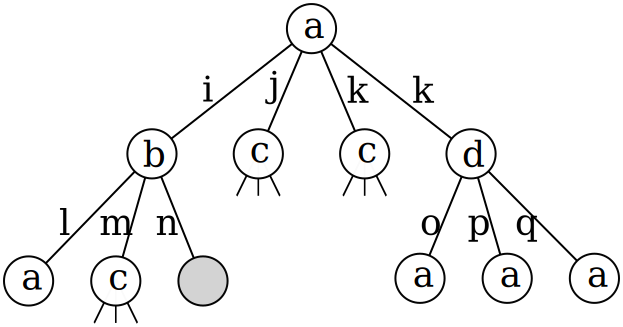
\includegraphics[width=.9\columnwidth]{figures/rotamersearch}
	\caption{The structure of our rotamer search space when eliminating
      collisions with the amino acid \textit{a}.}
    \label{fig:rotamer-search-tree}
\end{figure}
We have devised a simple algorithm for selecting side-chain rotamers,
with the goal of minimizing the number of collisions between
atoms. The first step of our algorithm is to apply the rotamer from the rotamer library
with highest probability to each amino acid in the protein. After
this, we go through each amino acid, this time trying to eliminate
eventual collisions. The search for collisionless rotamers can be
described by a tree, that represents the eventual collisions occuring
for each choice of rotamer for the amino acids. On Figure
\ref{fig:rotamer-search-tree} we have illustrated such a tree, for the
situation where we want to remove collisions with a single amino acid,
\textit{a}. Each vertex represents an amino acid and each edge
represents a collision between the node and its child. The names on
the edges represents rotamers of the node above. For example, when
the rotamer $3$ is applied to amino acid \textit{a}, \textit{a} collides
with both \textit{c} and \textit{d}.

We use a breadth-first search through the tree, visiting each level
down to some maximum depth. The edges are followed in order of
rotamer-probability, such that the most probable rotamer are visited
first (left-to right on the figure). We continue through the tree
until a solution (grey node in the figure) is found or the maximum
depth is reached. In the example on figure, we can eliminate the
collision by using rotamer $1$ for amino acid \textit{a} and rotamer
$3$ amino acid \textit{b}. In cases where an amino acid collides with
more than one other amino acid, we stop as soon one of the collisions
is solved and postpone the solution of the remaining collisions to we
reach one of the collidees we haven't handled.

%% Hvornår kigger vi på rotameren som /a/ startede ud med at have?

\section{Related Work}
The side-chain positioning (SCP) problem has been investigated by
several research groups, what we found most notably is the work done
by Dunbrack Labs on the SCWRL project \cite{canutescu2003graph,
  krivov2009improved}. The central algorithm in SCWRLs collision
resolving uses an \textit{interaction graph}, which much like our tree
has a vertex for each amino acid, but instead of the edges
representing that there currently is a collision, the graph has edges
between two amino acids if they \textit{could} collide by applying
certain rotamers on either or both of the amino acids. This graph can
be used to find clusters of interacting residues (two residues can
interact if there is a path between them). Large clusters cant be
solved efficiently, but they a cluster can be partitioned if there
exists what is called \textit{keystone vertices}
or\textit{articulation points} a which when removed breaks the graph
into two seperate subgraphs. For each rotamer of the keystone residue
the two subproblems can be solved. The rotamer of the keystone residue
which results in the lowest amount of free energy for the complete
cluster. Remark here that they use energies to evaluate the best
rotamer where as we have limited us from dealing with energy functions
and instead concentrate on the number of collisions.

In addition to this central algorithm, SCWRL has further advantages
over our algorithm. They use a lot of effort to delimit their search
space e.g. by removing rotamers with high self-energy from the set of
possible rotamers, where as we haven't focused at all on performance
in our implementation. SCWRL also tries to resolve whether any
collisions can be transformed into disulfide bridges, which are bonds
between two Cysteine amino acids (only pairs of Cysteine residues can
form disulfide bridges) from different places on the amino acid
sequence but spatially near each other. A problem we limited ourselves
from, from the beginning.

%%% Local Variables: 
%%% mode: latex
%%% TeX-master: "rapport"
%%% End: 
